\chapter{Choosing by looking}\label{ch:pictures}

\section{Why pictures}
Customers do not know the names of necklines, and tailors and customers often use the same word for different shapes. ``Straight'' on a kurta and ``straight'' on trousers are different cuts; ``fitted'' on a sweatshirt is not ``fitted'' on a blouse. Showing a drawing removes both problems. The attribute set is fixed by the ontology, so no live image search is needed: the pictures are made once, checked, and served as static files.

\section{The catalogue}
The catalogue has one entry for each value a question or the picker can offer: 47 garments, 18 necklines, four neckline depths, nine sleeve styles, six sleeve lengths, four fits, 14 silhouettes, seven lengths, 27 fabrics, 13 prints and 12 finishes, 171 in all. Where one word means two shapes, there is a second drawing in a context: fits drawn on a sweatshirt for knits, and silhouettes and lengths drawn on trousers for bottoms. The interface asks the engine which context the current design is in, using the same rule that chooses the question, so a customer designing joggers sees trouser shapes first. Every key is an ontology ID (\code{neckline.shape/sweetheart}, \code{lower.silhouette/straight@bottom}), so the tagger, the language-model layer, the picker and the tailor sheet all use the same names.

Garments and details are drawn as technical flat sketches: front view, uniform black outlines, no shading, no person, on white, the convention of a tailor's tech pack. Lengths need a body for reference and are drawn on a plain faceless croquis. Fabrics, prints and finishes are photographs, because texture does not survive as line art; fabrics are shown in ivory unless the fabric is defined by its colour (denim, tan leather), and prints in indigo on ivory, so that the set reads as one family.

\section{Generation}
The model is FLUX.2 [klein] 4B from Black Forest Labs \cite{bfl2026klein}, a four-billion-parameter rectified-flow transformer distilled to four sampling steps and released under Apache 2.0, which permits commercial use. It was chosen over FLUX.1 [schnell] \cite{bfl2024flux} for three reasons: it is a third of the size, it needs no account to download, and it can edit a reference image, which is what makes a consistent set possible. For details that should vary on an otherwise identical garment (necklines, sleeves, fits, lengths), a base sketch is drawn once and every option is an edit of it with the instruction to change only that part. The result reads like a library of variations on one pattern rather than unrelated drawings.

The card for the model asks for about 13\,GB of GPU memory; the laptop has 6\,GB. Streaming layers from system memory on every step worked but took about two minutes an image. The final pipeline splits the work instead (Figure~\ref{fig:looks}). Every prompt is encoded once by the 4B text encoder, streamed through the GPU one layer at a time in batches of eight, and the embeddings are cached on disk; this peaks at 2.6\,GB and takes 0.6\,s a prompt, where keeping whole blocks resident overflowed the card and took 9\,s. The encoder is then freed, and the transformer is loaded entirely onto the GPU with its weights stored as 8-bit floats and computed in bfloat16, about 4\,GB, so nothing moves between memories while sampling. A picture then takes 7.3\,s, sixteen times faster than streaming.

\begin{figure}[tbp]
\centering
\resizebox{\linewidth}{!}{\begin{tikzpicture}[x=1cm,y=1cm,
  st/.style={box,text width=2.35cm,font=\footnotesize,minimum height=1.55cm},
  hd/.style={font=\small\scshape,anchor=base},
  nb/.style={font=\scriptsize,text=soft,align=center,text width=2.5cm,anchor=north}]
\def\dx{2.85}
\foreach \i/\h/\f/\d/\t/\n in {
 0/catalogue/greyF/greyD/{171 options keyed by ontology IDs}/{one style sentence for every drawing},
 1/encode/blueF/blueD/{4B text encoder, every prompt once}/{streamed through the GPU, then freed},
 2/draw/lavF/lavD/{FLUX.2 [klein] 4B, 4 steps, 640 px}/{float8 weights on a 6 GB GPU},
 3/edit/lavF/lavD/{same base sketch, one detail changed}/{necklines, sleeves, fits, lengths},
 4/rank/sandF/sandD/{CLIP ViT-L/14 against all options in the group}/{plus penalties for clutter},
 5/review/roseF/roseD/{contact sheets, picks by hand}/{recorded in picks.json},
 6/publish/greenF/greenD/{ink on transparent, 384 px WebP}/{manifest shared with the engine}}{
  \node[hd] at (\i*\dx,0.95) {\h};
  \node[st,fill=\f,draw=\d] (s\i) at (\i*\dx,0) {\t};
  \node[nb] at (\i*\dx,-0.95) {\n};
}
\foreach \a/\b in {0/1,1/2,2/3,3/4,4/5,5/6}{\draw[flow] (s\a.east) -- (s\b.west);}
\end{tikzpicture}
}
\caption{How the picture library is made. Only the last step's output ships with the site; the raw variants stay on the machine that made them.}
\label{fig:looks}
\end{figure}

\begin{figure}[tbp]
\centering
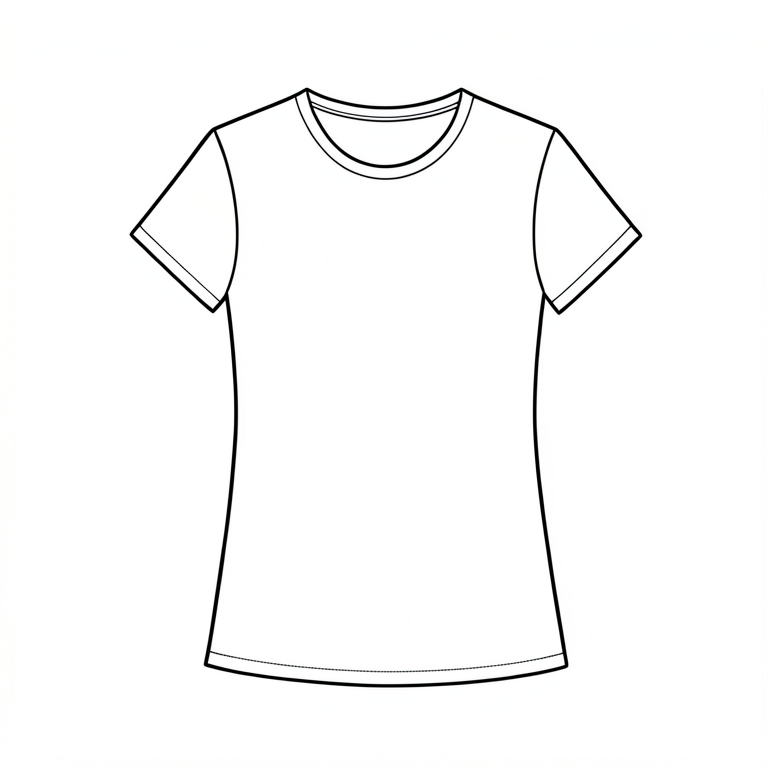
\includegraphics[width=0.36\linewidth]{img/base-top.png}
\caption{A base sketch from the first test run: a plain top drawn from the style sentence alone. Neckline and sleeve options are edits of a sketch like this one.}
\label{fig:base}
\end{figure}

\section{Ranking, review and cleaning}
Each option is drawn from two seeds: by editing its base where it has one, so the set stays consistent, and from text otherwise. CLIP ViT-L/14 \cite{radford2021clip} scores every variant against the descriptions of all options in its group, so a variant scores well only if it shows this option and not a neighbouring one; a sweetheart neckline that CLIP mistakes for a square one is ranked down. Line drawings that touch the edge of the frame or are mostly dark are penalised. Generators often draw necklines and sleeves wrongly, so the ranking is a first pass only: contact sheets of every option with its variants are reviewed by hand, and the choices are recorded in a file that the publishing step reads before it falls back to the ranking.

Publishing turns each sketch into ink on a transparent background (white becomes transparent, lines keep their weight), trims and centres it, and saves it as a 384\,px WebP; photographs are cropped square. The manifest maps each key to its file. A test checks that every file exists and is under 80\,kB, that every key is an ontology value, and that every question the assistant can ask, for every garment and season, can be answered by picture.

\section{Status}
The pipeline, the catalogue, the interface and the tests are complete, and the first base sketches show the intended style (Figure~\ref{fig:base}). The full library of 171 pictures is being generated and reviewed; until it is published, the interface falls back to the text choices it used before, option by option.
